%%%%%%%%%%%%%%%%%%%%%%%%%%%%%%%%%%%%%%%%%%%%%%%
\chapter{Decoding FEC Chain} \label{chap:DecodingChain}
%%%%%%%%%%%%%%%%%%%%%%%%%%%%%%%%%%%%%%%%%%%%%%%
In 5G Polar FEC chain, decoder is the critical part due to inherent sequential nature of polar decoding. $n^{th}$ bit is decoded by using all the previously decoded bits, hence $n^{th}$ bit depends on $0$ to $n-1$ bits. Due to sequential decoding process, significant latency is introduced by the decoder. This section presents the optimization techniques employed to improve the latency, which include both algorithmic and platform specific optimizations. Each these techniques are explained in the respective sections where these are employed. Polar decoder FEC chain is present at the receiver side. In this work, FEC chain considered is part of the base station therefore uplink control data is decoded at receiver. PUCCH (Physical uplink control channel) and PUSCH (Physical uplink shared channel) contain polar encoded information. Received signal after demodulation is quantized to 16-bit LLR (log likelihood ratio) values. Decoding is performed with LLR (Log likelihood ratio) values rather than probabilistic likelihoods due to their numerical stability and low computational complexity. Receiver side FEC chain is a reverse of the operations performed at transmitter. Figure ~\ref{fig:5grx_fec_chain} shows the receiver side polar decoding FEC chain.
\begin{figure}[]
	\centering
	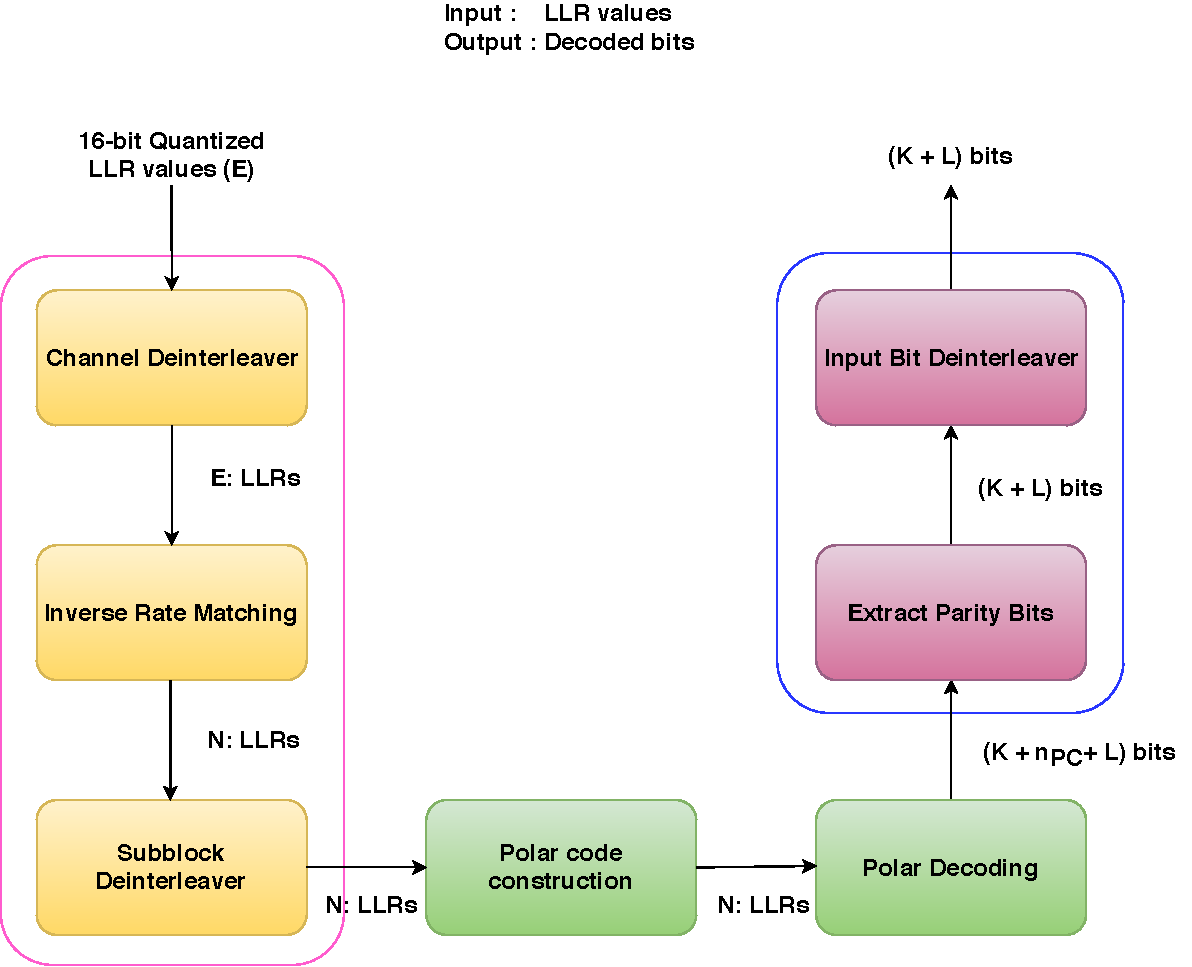
\includegraphics[width=0.7\textwidth]{./figures/receiverFECChain.pdf}
	\caption{Polar decoding FEC chain for PUCCH/PUSCH}
	\label{fig:5grx_fec_chain}
\end{figure}
%$\mathtt{Yadhu}$
%\NOTE{Decoding is of serial nature, has lot of latency. Polar decoding chain necessity. PUCCH and PUSCH, parameters of both the channels.}
%%	Explain all the decoding Optimizations I have done, In this document.
%% 	Explain of the latency without optimization.
\section{Decoding algorithms}
The basic decoding algorithm successive cancellation (SC) is developed by the Arikan in his seminal work on polar codes \cite{Arikan}. It achieves the symmetrical capacity of binary memoryless channel through sequential decoding when block length is very large. However due to the sequential nature significant latency is introduced by decoding algorithm. Latest 5G standard specifies transmission time interval (TTI) of $125 \mu s$ \TODO{cite the doc}, within this duration scheduling and encoding/decoding must be done. Therefore it is very important to efficiently perform FEC chain operations. This work concentrates on implementing the polar encoding/decoding in software and studies the feasibility of satisfying the strict latency requirements of 5G.

\section{Decoding chain}

\section{Sub-block de-interleaver}

\section{Inverse rate matching}

\section{Channel deinterlever}

\section{Decoder optimization}

\subsubsection{Bit packing frozen pattern}
How different kind of sub code types are identified efficiently using with bit packed frozen bits.

\subsubsection{Decoding Rate-1 code}

\subsubsection{Decoding SPC code}

\section{Extract Info Bits}
Means select information bits from the reliable positions.

\section{Remove parity check bits}


